% !TEX root = trkjet.tex

The analysis procedure is similar to the procedure in \cite{Aaboud:2018hpb} with the additional requirement of being done differentially in \rvar. Measured tracks are associated with a reconstructed jet if they fall within $\Delta R < 0.8$ of the jet axis and are constructed as:

\begin{eqnarray}
\dfrac{\fd^{2} \nchmeas }{ \fd \pttrk \fd r} = \frac{1}{\varepsilon(\pttrk,\etatrk)} \frac{\Delta \Nch( \pttrk, r)}{ \Delta\pttrk \Delta r}
\end{eqnarray}

where $\Delta \Nch (\pttrk, r)$ represents the number of tracks within a given \pttrk\ and $r$ range. The efficiency correction is applied as a $1/\varepsilon(\pttrk,\etatrk)$ weight on a track-by-track basis, assuming $\pttrk = \pTtrue$. While that assumption is not strictly valid, the efficiency varies sufficiently slowly with $\pTtrue$ that the error
introduced by this assumption is less than 1\%.

The measured track yields need to be corrected for the underlying event, fake tracks and secondaries. In \pp\ collisions, the UE contribution from hard scatterings not associated with jet production is negligible. The contributions from fake tracks and secondary charged particles are estimated from MC samples and subtracted. This procedure is similar to previous measurements~\cite{Aaboud:2017tke,Aaboud:2018hpb}.

For \pbpb\ collisions, the UE, fake track, and secondary contributions are estimated together in a two step process: first, MC overlay are used to generate \etajet--\phijet maps of the average number of charged particles in a given annulus around a reconstructed jet. This is done for charged particles without a truth match and as a function of \ptjet, \etajet, \phijet, angle of the jet to the second order event plane\footnote{The second order event plane angle $\Psi_2$ is determined on an event-by-event basis by a standard method using the $\phi$ variation of transverse energy in the forward calorimeter \cite{ATLAS:2012at}} $ \mathrm{d}\Psi_{\mathrm{jet}}$, \rvar, \pttrk, and centrality. In the second step, the \etajet--\phijet maps are used to generate the underlying event distribution for jets with a given \etajet, \phijet, and $\mathrm{d}\Psi_{\mathrm{jet}}$. This distribution includes fakes, and is given by \mbox{$\fd^2 \nch^{\mathrm{UE+Fake}}(r) / \fd \pttrk \fd r$}. The yields decrease with the decreasing collision centrality, increasing \pttrk, and increasing azimuthal distance from $\Psi_2$. The subtracted distributions are then given by 

\begin{align}
\frac{\fd^2 \nchsub }{ \fd \pttrk \fd r } &=  \frac{\fd^2 \nchmeas }{ \fd \pttrk \fd r} -  \frac{ \fd^2 \nch^{\mathrm{UE+Fake}}(r)  }{ \fd \pttrk \fd r} 
\end{align}

Figure~\ref{fig:UEsize} shows the ratio of the charged-particle distributions before and after the UE and fake track subtraction,
%the charged-particle distributions prior to the UE and fake track subtraction, $ \fd^2 \nchmeas / \fd \pttrk \fd r$, divided by the distributions after the subtraction, $ \fd^2 \nchsub / \fd \pttrk \fd r $
 as a function of \rvar\ for different \pttrk\ intervals and $126 < \ptjet < 158$ \GeV\ for six centrality selections. The UE contribution is the highest for 1.0~\GeV\ charged particles at large values of \rvar\ and in central collisions, with the signal to background being approximately 1:100. It is rapidly decreasing towards more peripheral collisions, larger \pttrk\ and smaller \rvar. Furthermore, the signal to background
slowly increases with increasing \ptjet.

\begin{figure}
\centerline{
 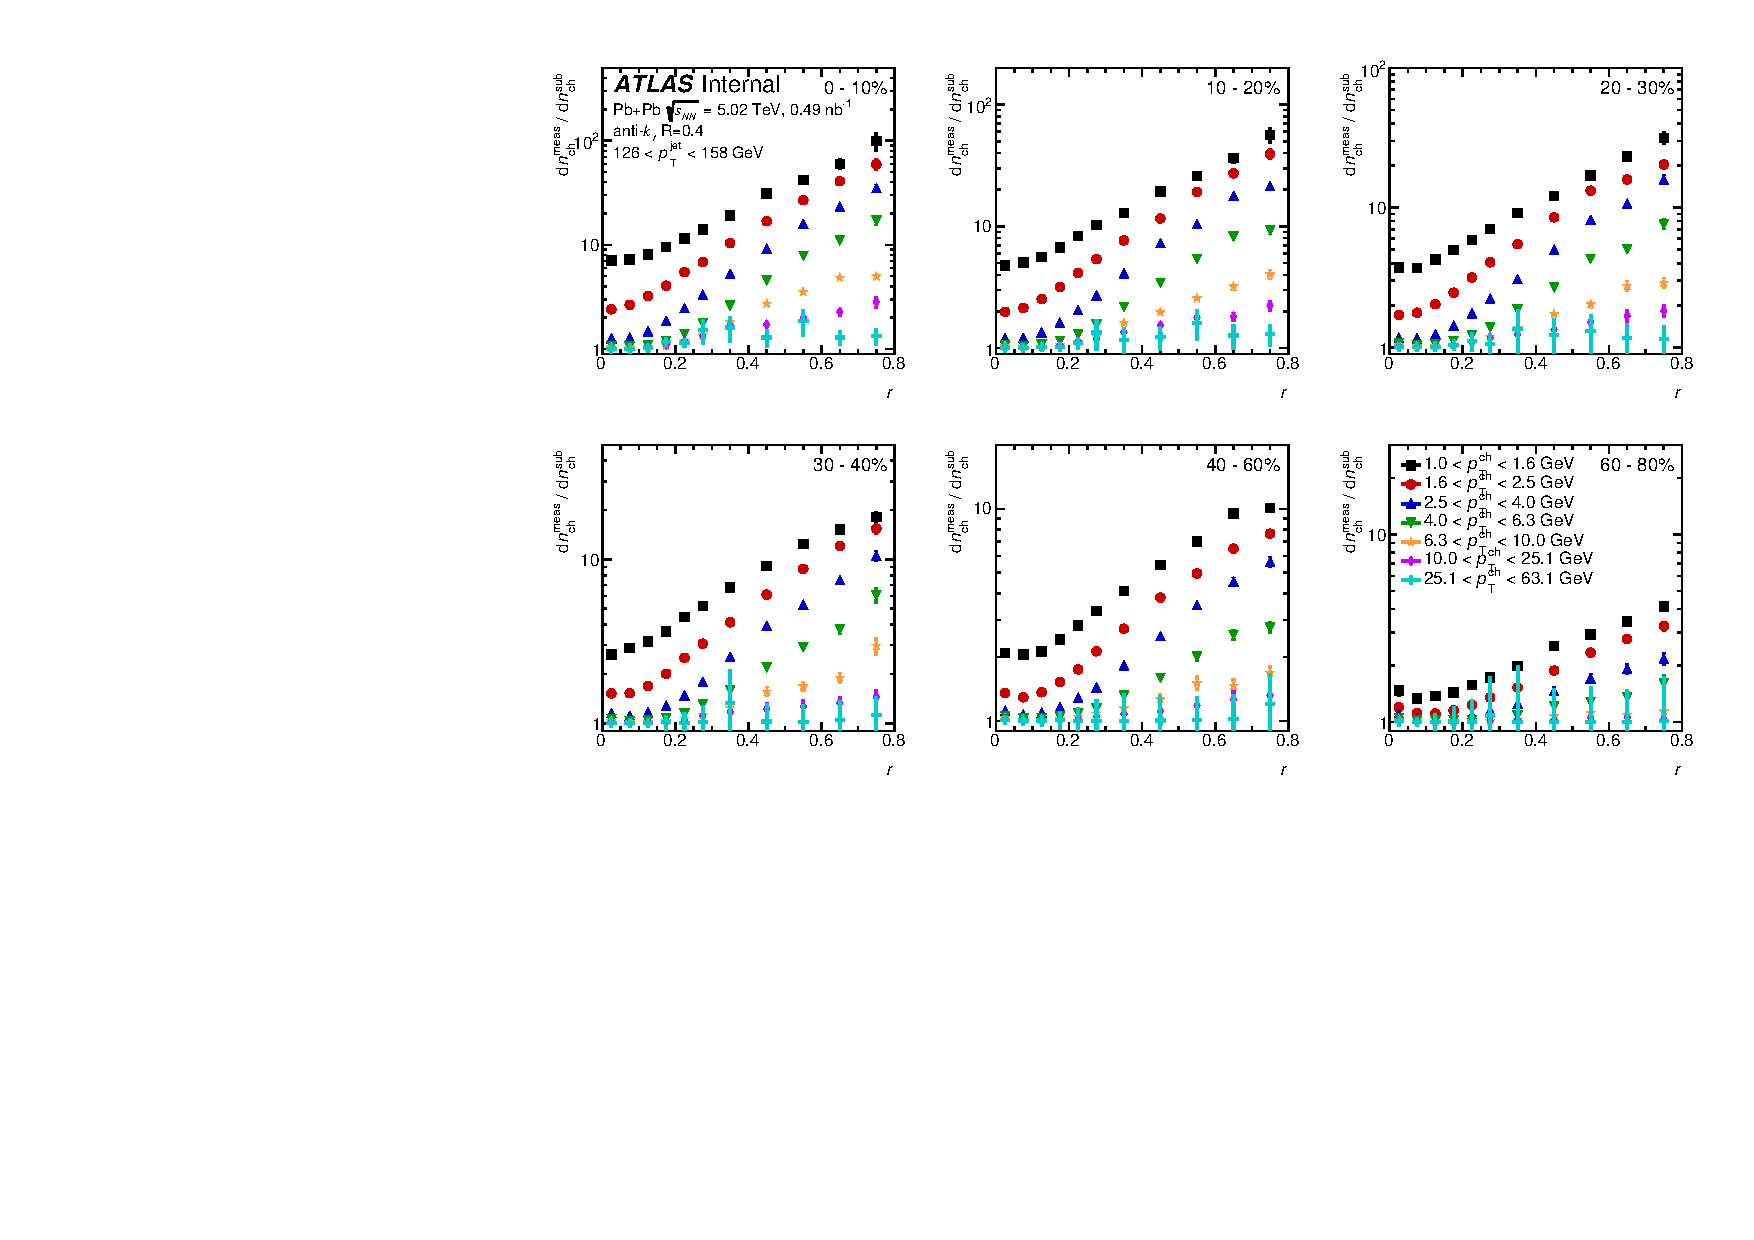
\includegraphics[width=0.95\textwidth]{figures/performance/UE_B2S_single_0.pdf} }
\caption{ Ratio of the raw charged particle distributions to those after the subtraction of the UE and fake tracks as a function of \rvar\ for different \pttrk\ intervals, six centrality selections and for \ptjet\ between 126--158~\GeV.}
\label{fig:UEsize}
\end{figure}


%The fraction of fake tracks is found to be below 2\% of the tracks that pass the selection in all track and jet kinematic regions in this analysis.

To remove the effects of the bin migration due to the jet energy and track momentum resolution, the subtracted $\fd^2 \nchsub /\fd\pttrk \fd r$ distributions are corrected by a two-dimensional Bayesian unfolding~\cite{DAgostini:1994zf}
in \pttrk\ and \ptjet\ as implemented in the RooUnfold package~\cite{Adye:2011gm}.  
Two-dimensional unfolding is used because the calorimetric jet energy response depends on the fragmentation pattern of the jet~\cite{Aad:2011he}.
Four-dimensional response matrices are created from the \pp\ and \pbpb\ MC samples using the generator-level and reconstructed \ptjet, and the generator-level and reconstructed charged-particle \pttrk. They are corrected for tracking efficiencies and are evaluated in bins of \rvar\ and centrality. The Bayesian procedure requires a choice in the number of iterations.
Additional iterations reduce the sensitivity to the choice of prior, but may
amplify statistical fluctuations in the distributions.
After four iterations the 
charged particle distributions are found to be stable for both the \PbPb\ and \pp\ data.
A separate one-dimensional Bayesian unfolding is used to correct the measured \ptjet\ spectra that are used to normalize the unfolded charged particle distributions.
To achieve better correspondence with the data, the response matrices for both the one and two dimensional unfolding are reweighted so that the distributions match the shapes in the reconstructed data.

An independent bin-by-bin unfolding procedure is also used to correct for migrations originating from the finite jet and track angular resolutions. Two corresponding \Dptr\ distributions are evaluated in MC samples, one using generator-level jets and primary particles and the other using reconstructed jets and charged particles with their reconstructed \pt\ replaced by generator-level transverse momentum, \pTtrue. The ratio of these two MC distributions provides a correction factor which is then applied to the data. 

The final particle-level corrected distributions, normalized by the area of the annulus under question are defined as:
\begin{eqnarray}
 \label{eq:Dpt}
   \Dptr = \frac{1}{N_\mathrm{jet}^\mathrm{unfolded}} \frac{1}{A(r)} \frac{\fd^2 \nchunf(r)}{\fd \pt \fd r},
 \end{eqnarray}
where $\text{N}_{\text{jet}}^{\text{unfolded}}$ is the unfolded number of jets in a given \ptjet\ interval.

The performance of the full analysis procedure is validated in the MC samples by comparing the fully corrected charged particle distributions to the generator-level distributions. Good closure (< 3\%) is seen for charged particles with $\pt < 10$ GeV
Adding or removing particles carrying a large fraction of the jet momentum near the edge of the jet can significantly alter its
reconstructed momentum and position; this instability leads to a non-closure in the analysis procedure.
Results are presented where the non-closure in the \pp\ MC sample is less than 5\%.

%, excluding the following regions of phase space: 6--10 GeV tracks above $\rvar > 0.3$, 10--25 GeV tracks above $\rvar > 0.3$, and 25--63 GeV tracks above $\rvar > 0.2$ for 126--158 GeV jets; 10--25 GeV tracks above $\rvar > 0.4$, and 25--63 GeV tracks above $\rvar > 0.3$ for 158--200 GeV jets; 25--63 GeV tracks above $\rvar > 0.3$ for 200--251 GeV jets.



